\subsection{Builder}

\textbf{Definición:} El patron builder o constructor tiene el objetivo de permitir la creación de objetos complejos mediante un intermediario mas simple que encapsule la lógica asociada a la creación del objeto requerido.

\textbf{Motivación:} Por lo general, los lenguajes orientados a objetos permiten la creación de nuevas instancias de un objeto a través del uso de constructores y facilitan la definición de sus propiedades mediante el uso de su setter. Sin embargo, en algunas ocasiones un objeto puede tener múltiples combinaciones de sus propiedades o necesita ser inmutable, para estos casos la solución mas común es crear constructores específicos para cada combinación o mediante funciones que se encarguen de fijar sus atributos. Esto no es incorrecto y corresponde al diseño orientado a objetos, pero trae como desventaja que con el tiempo el código resultante sea demasiado extenso dificultando su mantenimiento.

\textbf{¿Como puedo implementar un builder?:} El patrón define una clase Builder cuyo objetivo es encapsular toda la lógica necesaria para crear el objeto. Particularmente, JAVA utiliza un builder muy conocido y utilizado por los desarrolladores (la clase StringBuilder) que encapsula toda la lógica involucrada en la creación de Strings complejos.

\textbf{Escenarios de aplicación:}

\begin{itemize}
	\item Existen muchas configuraciones posibles para la creación de un objeto.
	\item Se desea prescindir de multiples constructures en la implementación.
	\item La creación de un objeto complejo debe ser independiente de las partes que lo componen y debe ser lo suficientemente genérica para soportar múltiples representaciones del objeto.
	\item Crear una estructura genérica para facilitar los test de una clase.
	\item El objeto que se va a construir es inmutable
\end{itemize}

\textbf{Modelo UML:}

El patrón se centra en la definición de una clase Builder encargada de crear la estructura del objeto que se pretende construir. El truco fundamental para la abstracción del builder es la definición de métodos públicos que asocien cada propiedad al objeto y retornen la instancia del builder, lo cual permite que el objeto sea construido de manera dinámica de acuerdo a la necesidad del usuario. Finalmente, el builder cuenta con un método \textbf{build()} que se retorna la instancia del nuevo objeto al usuario.

\begin{figure}[H]
	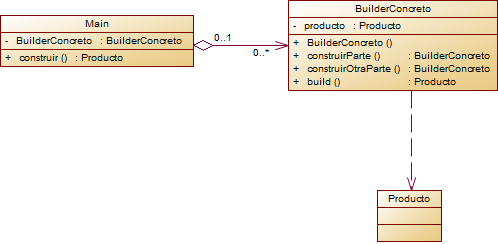
\includegraphics[width=0.9\textwidth]{images/creational/builder/builder.png}
\end{figure}

\textbf{Ejemplo conceptual:} En física, la teoría de cuerdas propone la existencia de múltiples Universos, cada uno con sus propias propiedades físicas inmutables.

Se solicita a un desarrollador crear un programa computacional que simule la creación de Universos de una manera sencilla y compacta. Para simplificar el problema, asumiremos que un Universo puede ser caracterizado en función de: un identificador, un código único, su masa, el porcentaje de materia barionica que posee (la materia barionica es la materia de la cual estamos compuestos), su porcentaje de materia oscura y su porcentaje de energía oscura (en física y en astronomía se da el indicativo de oscuro a todo aquello que no tenemos la mas remota idea de que pueda ser), y sus galaxias.

En general, cualquier objeto puede ser identificado a partir de un id y código únicos, por ello se crea una clase General que nos permita obtener estos atributos para cualquier clase en el dominio de la aplicación.

\begin{figure}[H]
	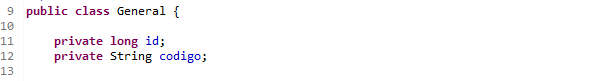
\includegraphics{images/creational/builder/builderExample1.png}
\end{figure}

Adicionalmente, se crea la estructura necesaria para crear nuevos Universos. Finalmente se extiende de la clase General para obtener los atributos comunes.

\begin{figure}[H]
	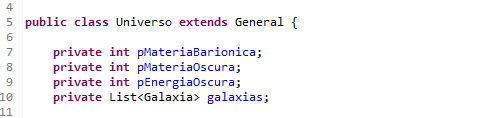
\includegraphics{images/creational/builder/builderExample2.png}
\end{figure}

De manera análoga, se crea la estructura necesaria para crear nuevas galaxias (cada galaxia podría tener a su vez estrellas que contengan planetas, pero eso no nos interesa por ahora).

\begin{figure}[H]
	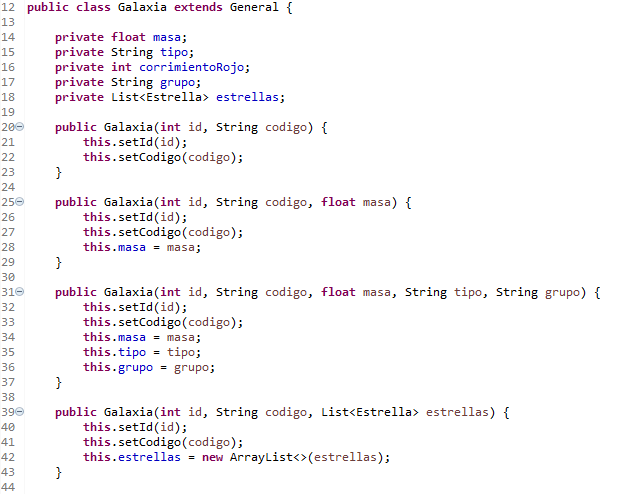
\includegraphics{images/creational/builder/builderExample3.png}
\end{figure}

 Como se puede observar, se decidió deliberadamente definir varios constructores en la clase Galaxia para ilustrar un punto. Sin la definición de un builder, cada vez que se quiera crear una nueva galaxia con características particulares sería necesario crear un nuevo constructor o fijar cada atributo uno a uno a través de sus metodos get. Esto es poco práctico y con el paso del tiempo la clase se comienza a hacer bastante extensa dificultando su mantenimiento. Por ahora nos enfocaremos en un builder para nuestro Universo, mas adelante buscaremos el mecanismo para crear nuevas galaxias de una manera mas adecuada.
 
 Por otro lado, se define una clase UniversoBuilder que a su vez contendrá el Universo en cuestión. Inicialmente, se crea la estructura básica con un constructor que inicialice los atributos obligatorios y los valores por defecto.
 
 \begin{figure}[H]
	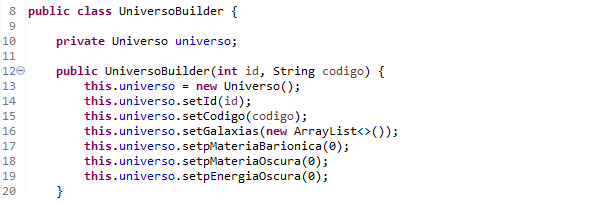
\includegraphics{images/creational/builder/builderExample4.png}
\end{figure}
 
 La clave para la implementación del patrón es la definición de métodos públicos que se encarguen de llenar el objeto y retornen el builder, esto permitirá la construcción del objeto de manera dinámica y garantizará que se pueda construir el objeto de acuerdo a las necesidades del usuario. Finalmente, se define un método build que retornará nuestro nuevo Universo.
 
 \begin{figure}[H]
	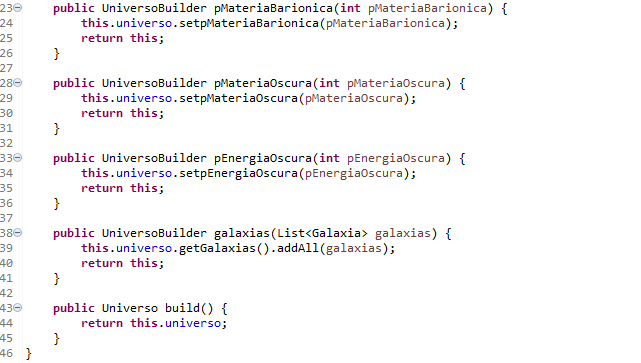
\includegraphics{images/creational/builder/builderExample5.png}
\end{figure}
 
 Gracias a esto, una clase externa ahora puede crear Universos de una manera compacta y de acuerdo a su necesidad.
 
 \begin{figure}[H]
	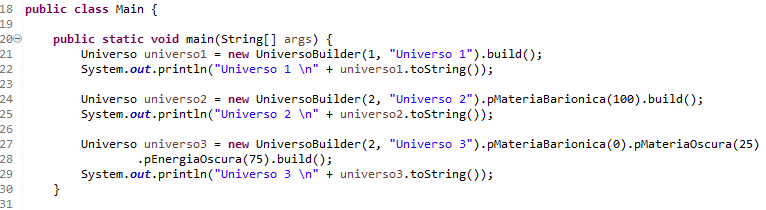
\includegraphics{images/creational/builder/builderExample6.png}
\end{figure}
 
 \begin{figure}[H]
	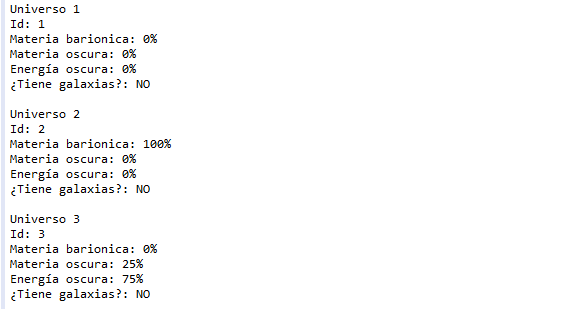
\includegraphics{images/creational/builder/builderExample7.png}
\end{figure}

Hasta ahora las cosas van bastante bien ¿pero que pasaría si necesitaramos crear nuevas galaxias? Supongamos que queremos crear un nuevo Universo con varias galaxias de diferentes características. De acuerdo a la definición actual se tendría que llamar un constructor diferente para cada configuración o crear el objeto y fijar sus atributos uno a uno, lo cual es poco práctico.

\begin{figure}[H]
	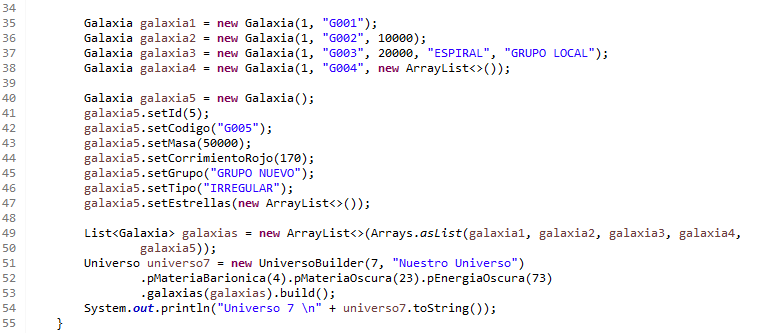
\includegraphics{images/creational/builder/builderExample8.png}
\end{figure}

Sin embargo, se puede definir una clase GalaxiaBuilder encargada de simplificar la creación de los objetos y prescindir de los constructores en el objeto original. Gracias a esto, la instanciación de nuevas Galaxias se haría desde el builder.

\begin{figure}[H]
	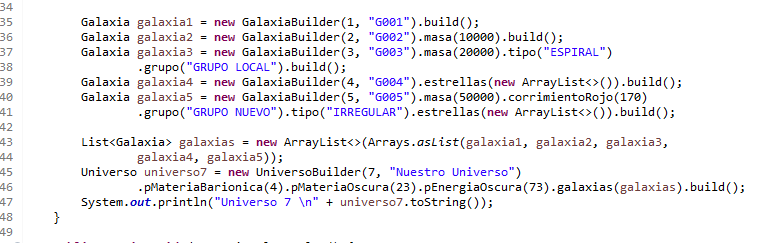
\includegraphics{images/creational/builder/builderExample9.png}
\end{figure}

Como resultado, el builder permite abstraer la construcción de cualquier combinación del objeto a una estructura mas compacta. Inicialmente podría pensarse que no hay una diferencia sustancial con respecto a la definición inicial, pero la ventaja del builder radica en eliminar la definición de multiples constructores y hacer el código mas fácil de comprender y mantener. Como resultado, la clase Galaxia ya no necesita constructores.

\begin{figure}[H]
	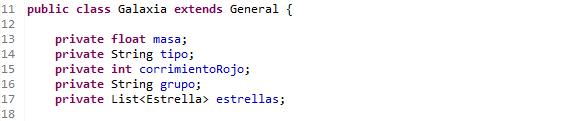
\includegraphics{images/creational/builder/builderExample12.png}
\end{figure}

Uno de los aspectos mas interesantes del patrón builder es que gracias a su flexibilidad puede implementarse de varias formas. A continuación, se presentará otra forma en la cual se podría resolver el problema presentado anteriormente. Para ello, se cambia la definición del builder a una clase estática contenida en el objeto que vamos a construir, en este caso nuestro Universo.

\begin{figure}[H]
	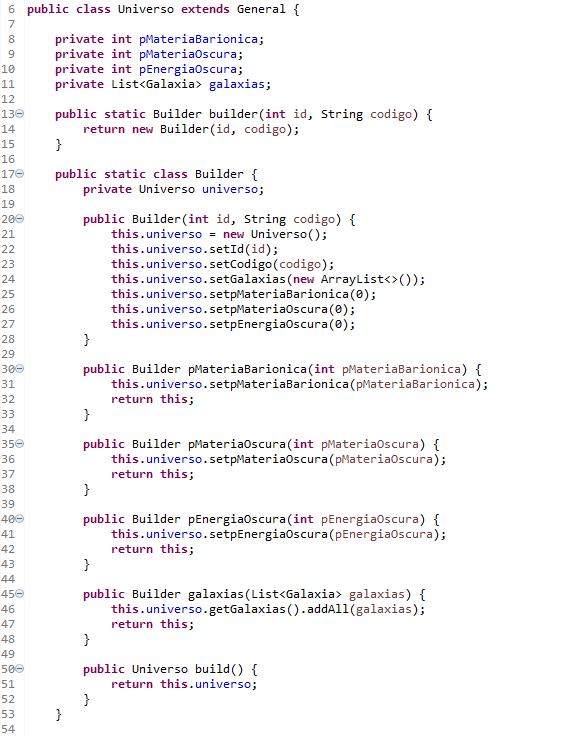
\includegraphics{images/creational/builder/builderExample13.png}
\end{figure}

De manera analoga, se crea la clase Galaxia con su propio builder. El aspecto mas importante que se debe considerar al utilizar esta aproximación es la definición de un constructor estático que permita la creación del builder contenido en la clase y que se va a encargar de construir el objeto.

\begin{figure}[H]
	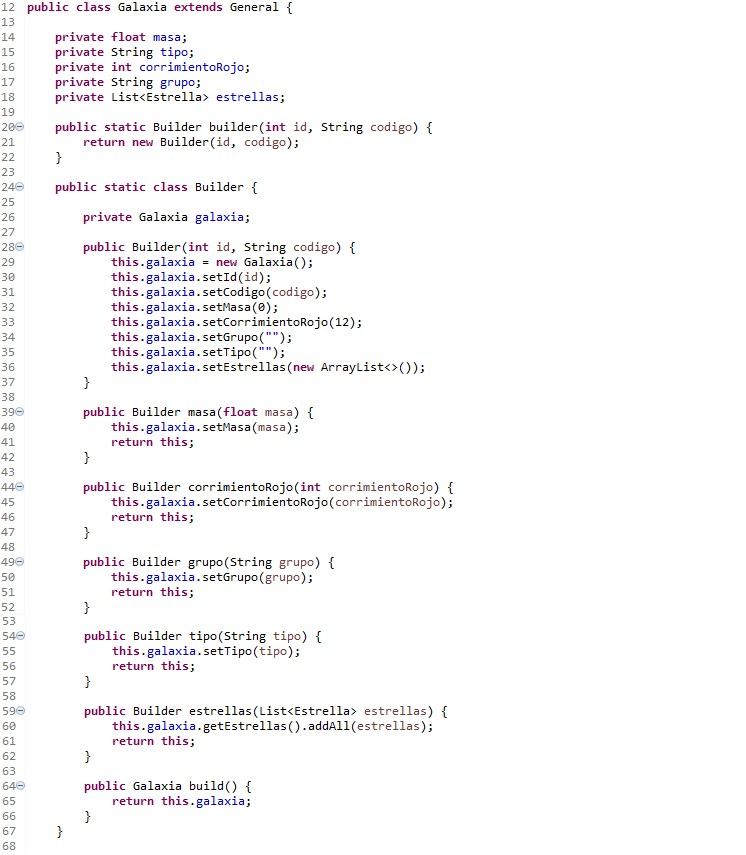
\includegraphics{images/creational/builder/builderExample14.png}
\end{figure}

Debido a que cada builder está acoplado al objeto que se va a crear es posible instanciar el objeto directamente desde la clase de manera estática.

\begin{figure}[H]
	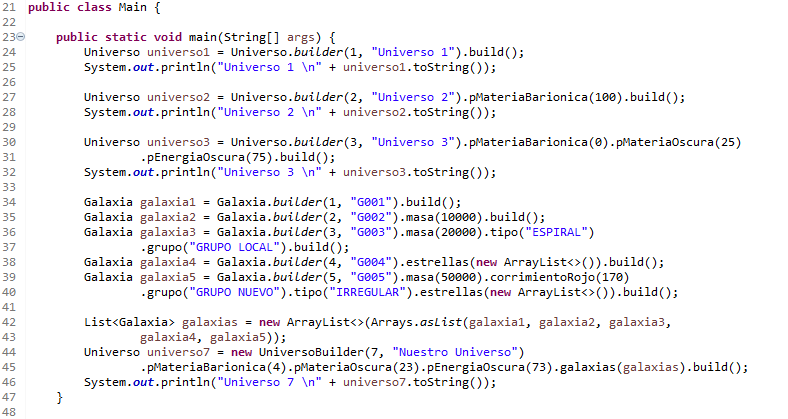
\includegraphics{images/creational/builder/builderExample15.png}
\end{figure}

Un aspecto interesante del patrón builder es su flexibilidad al permitir que su implementación sea realizada de diferentes maneras, en este libro se presentaron dos aproximaciones frecuentemente utilizadas en muchos frameworks. Sin embargo, otros autores como el Gof o Eric y Elizabeth Freeman presentan aproximaciones diferentes a esta, invito a cualquier lector curioso a indagar sobre las diferentes maneras de implementar el patrón builder. 

En este punto ya hemos logrado implementar el patrón builder y descubrimos que tiene grandes ventajas en la construcción de objetos complejos. Sin embargo, este patrón no debe ser utilizado a la ligera y el analisis de cuando debería usarse recae en la solución que se esté llevando a cabo. Se debe tener en cuenta que el patrón hace el código mas flexible con un costo (se requiere una clase adicional que aumenta el consumo de recursos en la aplicación). Es criterio del desarrollador decidir cuando el patrón builder es la mejor opción.